\documentclass[utf8]{beamer}
\usepackage[ngerman]{babel}
\usefonttheme{professionalfonts}
%\usetheme{Madrid}
%\usetheme{AnnArbor}
%\usetheme{CambridgeUS}

\begin{document}

\title[Kurztitel]{Dies ist der Titel des Vortrags}
\subtitle{Und hier der Untertitel}
\author{Max Meier}
\date{\today}
\institute{"`Universit"at Rostock"'}

\begin{frame}
	\titlepage
\end{frame}

\begin{frame}\frametitle{Inhalt}

Muss eigentlich nicht sein.

	\tableofcontents[pausesections]

\end{frame}

\section{Hello}

\begin{frame}\frametitle{Hello World}

\begin{itemize}

	\item Bullet 1
	\pause
	\item Bullet 2
	\pause
	\item Bullet 3

\end{itemize}

\end{frame}

\section{Once}

\begin{frame}\frametitle{Once Upon A Time}

\begin{enumerate}

	\item Bullet 1
	\pause
	\item Bullet 2
	\pause
	\item Bullet 3

\end{enumerate}

\end{frame}

\section{Einige Beispielfolien}

\begin{frame}
  \frametitle{There Is No Largest Prime Number}
  \framesubtitle{The proof uses \textit{reductio ad absurdum}.}
  \begin{theorem}
    There is no largest prime number.
  \end{theorem}
  \begin{proof}
    \begin{enumerate}
    \item<1-| alert@1> Suppose $p$ were the largest prime number.
    \item<2-> Let $q$ be the product of the first $p$ numbers.
    \item<3-> Then $q+1$ is not divisible by any of them.
    \item<1-> Thus $q+1$ is also prime and greater than $p$.\qedhere
    \end{enumerate}
  \end{proof}
\end{frame}


\subsection{Mathemodus}
\begin{frame}{Mathemodus und Fu{\ss}noten}{Funktionieren auch}
  Ein wenig Text\footnote{eine sinnfreie Fu{\ss}note} und ein wenig Mathematik im Sinne von
   \begin{align}
        V_{ab}^s\left(q, i z_\mu\right)
              &= \frac{V_{ab}(q)}{1-\sum_{c}V_{cc}(q)\Pi_{cc}\left(q, i z_\mu\right)} 
              \equiv \frac{V_{ab}(q)}{\varepsilon\left(q, i z_\mu\right)}  \\
          \rule{0pt}{2em}\varepsilon\left(q, iz_\mu\right) 
              &= 1-\sum_c V_{cc}(q)\Pi_{cc}\left(q, i z_\mu\right)
   \end{align}
   heitern diese Folie auf.
\end{frame}


\subsection{Aufz\"ahlungen}
\begin{frame}{Auflistungen und Aufz\"ahlungen}
   Diese Folie hat zur Abwechslung mal keinen Untertitel, daf\"ur ist sie aber zweispaltig.

   \begin{columns}
      \column<2->{0.45\textwidth}
         \begin{itemize}
            \item erster Auflistungspunkt
                  \begin{itemize}
                     \item n\"achste Ebene
                     \item n\"achste Ebene
                           \begin{itemize}
                              \item tiefste Ebene
                              \item tiefste Ebene
                           \end{itemize}
                     \item n\"achste Ebene
                  \end{itemize}
            \item zweiter Auflistungspunkt
         \end{itemize}

      \column<1->{0.45\textwidth}
         \begin{enumerate}
            \item mit Aufz\"ahlungen
                  \begin{enumerate}
                     \item geht das nat\"urlich
                           \begin{enumerate}
                              \item ebenso
                              \item wie mit
                           \end{enumerate}
                     \item Auflistungen
                  \end{enumerate}
         \end{enumerate}
   \end{columns}

\end{frame}


\begin{frame}{Auflistungen und Aufz\"ahlungen}
	Spalten mit Bildern
	\begin{columns}[T]

	\column<2->{.32\textwidth}
	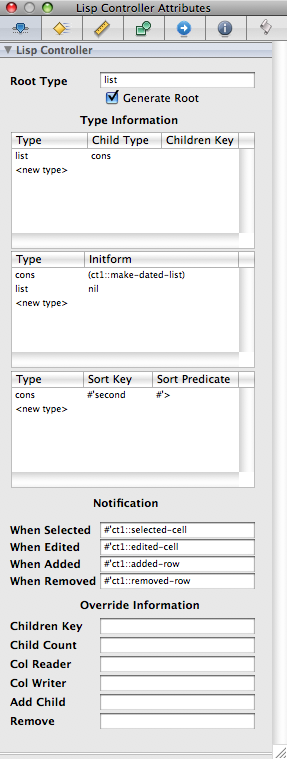
\includegraphics[width=\textwidth]{Controller10}
	\column<3->{.32\textwidth}
	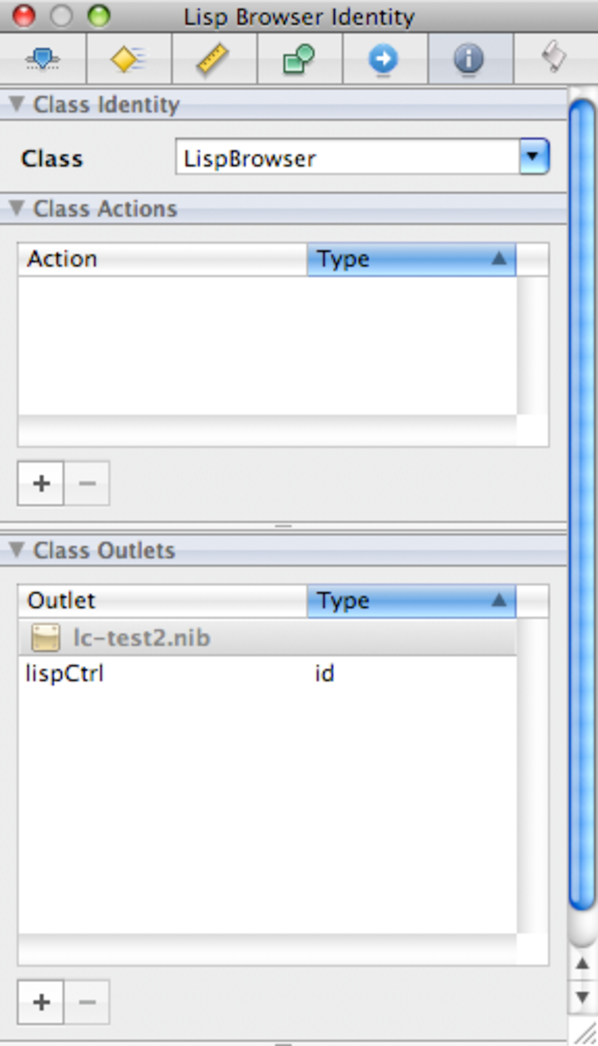
\includegraphics[width=\textwidth]{Controller12}
	\column<4->{.32\textwidth}
	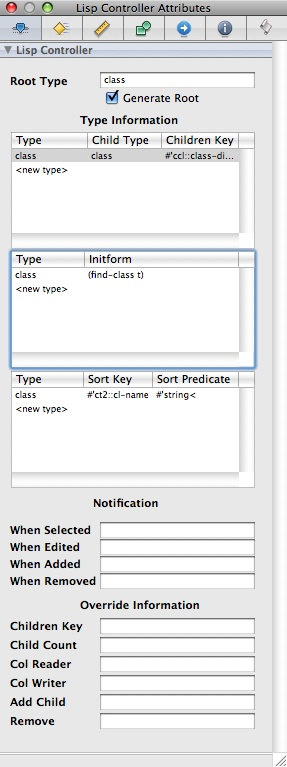
\includegraphics[width=\textwidth]{Controller13}

	\end{columns}
\end{frame}

\begin{frame}{Blah}
Nothing to see here.
\end{frame}

\subsection{Theorem / Beweis / andere Boxen} 

\begin{frame}[allowframebreaks]{Theorem / Beweis / andere Boxen} % Dieses Frame wird je nach Platz/Inhalt/Fuellstand automatisch geteilt
   \begin{theorem}
      Diese Box ist sch\"on.
   \end{theorem}

   \begin{proof}
      Die CD-Vorlage ist insgesamt schick, ergo muss jedes Teil hiervon dekorativ sein, folglich also auch die obige Theorem-Box.
   \end{proof}

   \begin{example}
     Diese Box ist auch ein nettes Beispiel f\"ur schicke Boxen.
   \end{example}

   \begin{block}{Blocktitel}
      Ein Block mit dem Titel \insertblocktitle
   \end{block}

   \begin{alertblock}{Alertblocktitel}
      Ein Alertblock.
   \end{alertblock}

   \begin{exampleblock}{Beispielblocktitel}
      Ein Beispielblock.
   \end{exampleblock}

\end{frame}


\end{document}
